% 使用 ExBook 文档类,并传递选项
\documentclass[standard]{ExBook} 
\usepackage{etoolbox} % 新增
\usepackage{forest}
\usepackage{pifont}

\begin{document}

% 加载配置  
% 封面设置
\CoverImg{img/cov01.jpg} % 封面图片
\PreTitle{ExBook · 刷题本模板} % 前置标题
\Title{此处填写主标题} % 主标题
\TitleDescription{此处填写副标题} % 副标题
\TypeOne{A4紧凑版} % A4紧凑版下的类型标识
\TypeTwo{A4标准版} % A4标准版下的类型标识
\TypeThree{横版Pad版} % 横版Pad版下的类型标识
\TypeFour{A4宽松版} % A4宽松版下的类型标识
\TypeFive{A4单题版} % A4单题版下的类型标识
\TypeSix{竖版Pad版} % 竖版Pad版下的类型标识
\motto{你这个年龄是怎么睡得着觉的} % 封面座右铭
\Creator{研小布} % 制作人
\UpdateTime{\today} % 更新时间

% 页眉页脚设置
\Lhead{微信公众号·研小布} % 左页眉 
\Chead{2025考研} % 中页眉、平板模式(padl或padp)下页眉中间的文字
\Rhead{408WD数据结构选择题刷题本} % 右页眉、平板模式(padl或padp)下页眉右侧的文字
\LheadC{公众号·研小布·} % 平板模式(padl或padp)下页眉左侧的文字

% 水印设置
\TextWater{【微信公众号·研小布】} % 文字水印 出现在题目后面
\WaterImg{img/water.png} % 图片水印 出现在页面的右下角

% 主题颜色设置,可选主题有:
% blue (默认)
% green
% purple
% orange
% infj
% enfp
% infp
% esfp
% intj
% entp
% isfj
% enfj
\setThemeColor{\orange}

% 加载封面
% \maketitle 
 
% % 加载声明
% \clearpage
\vspace*{0mm} % 添加两厘米的垂直空白
\begin{center}
    \large \heiti 前言
\end{center}

% \hspace*{2em}此刷题本依据 \underline{\textbf{\preBookName}}重新排版制作而成! 


\hspace*{2em}此刷题本的目的是方便大家在考研备考中多次刷题、记录自己的刷题过程和笔迹,以便日后复盘与巩固!
此刷题本不包含答案,答案请参考原书!

\hspace*{2em}关于其他考研刷题本的更新,请关注 \faWeixin 微信公众号:\underline{\textbf{研小布}},可使用微信扫描下面的二维码关注:


\begin{minipage}[t]{1.0\textwidth}
    \centering
    
\includegraphics[width=0.32\textwidth]{img/qr01.jpg} 
\end{minipage}

\hspace*{2em}如果你有\textbf{25考研数学}或者\textbf{专业课}清晰的PDF,可以投稿给小布,我来帮助制作刷题本,投稿微信:\textbf{\texttt{shang\_an\_001}}

\hspace*{2em}最后,希望此刷题本能够让你更高效地刷题,上岸值 ++ !祝考研顺利。
\clearpage 

% % 加载广告
% \clearpage
\hideheaderfooter

\vspace*{-5mm} 
\begin{center}
    \large \heiti 打印纸质版说明\footnote[1]{此说明只针对A4版做题本(A4标准版、A4宽松版、A4紧凑版、A4单题版)}
\end{center}

\hspace*{2em}\heiti{打印参数建议~~} \songti{A4纸张、黑白(或彩色)、双面(或单面) }

\hspace*{2em}\heiti{打印渠道推荐~~} \songti{微信扫描下方二维码进入小程序可进行在线打印,超优惠打印价格!70gA4纸单面0.07元/张,
双面0.05元/张。}

\vspace*{4em}

\imgin[0.28]{}{img/print.png}

\clearpage

\setcounter{page}{1}
% \tableofcontents 
    
% \clearpage 

% \setcounter{section}{1} 
% \section{线性表}
% \setcounter{subsection}{1}
% \begin{qitems}

    \begin{bbox}
        \qitem 从顺序表中删除具有最小值的元素 (假设唯一) 并由函数返回被删元素的值。空出的位置由最后一个元素填补,若顺序表为空,则显示出错信息并退出运行。
    \end{bbox}

    \begin{bbox}
        \qitem 设计一个高效算法,将顺序表 L 的所有元素逆置,要求算法的空间复杂度为 O(1)。
    \end{bbox}

    \begin{bbox}
        \qitem 对长度为 $n$ 的顺序表 $L$, 编写一个时间复杂度为 $O(n)$、空间复杂度为 $O(1)$ 的算法,该算法删除顺序表中所有值为 $x$ 的元素。
    \end{bbox}

    \begin{bbox}
        \qitem 从顺序表中删除其值在给定值 $s$ 和 $t$ 之间 (包含 $s$ 和 $t$, 要求 $s<t$) 的所有元素,若 $s$ 或 $t$ 不合理或顺序表为空,则显示出错信息并退出运行。
    \end{bbox}

    \begin{bbox}
        \qitem 从有序顺序表中删除所有其值重复的元素,使表中所有元素的值均不同。
    \end{bbox}

    \begin{bbox}
        \qitem 将两个有序顺序表合并为一个新的有序顺序表,并由函数返回结果顺序表。
    \end{bbox}

    \begin{bbox}
        \qitem 已知在二维数组 $A[m+n]$ 中依次存放两个线性表 $(a_1,a_2,a_3,\dots,a_m)$ 和 $(b_1,b_2,b_3,\dots,b_n)$。编写一个函数,将数组中两个顺序表的位置互换,即将 $(b_1,b_2,b_3,\dots,b_n)$ 放在 $(a_1,a_2,a_3,\dots,a_m)$ 的前面。
    \end{bbox}

    \begin{bbox}
        \qitem 线性表 $(a_1,a_2,a_3,\dots,a_n)$ 中的元素递增有序且按顺序存储于计算机内。要求设计一个算法,完成用最少时间在表中查找数值为 $x$ 的元素,若找到,则将其与后继元素位置相交换,若找不到,则将其插入表中并使表中元素仍递增有序。
    \end{bbox}

    \begin{bbox}
        \qitem 给定三个序列 $A、B、C$,长度均为 $n$, 且均为无重复元素的递增序列,请设计一个时间上尽可能高效的算法,逐行输出同时存在于这三个序列中的所有元素。例如,数组 $A$ 为 $\{1,2,3\}$, 数组 $B$ 为 $\{2,3,4\}$, 数组 $C$ 为 $\{-1,0,2\}$, 则输出 $2$。要求:
        \begin{subqitems}
            \subqitem 给出算法的基本设计思想。
            \subqitem 根据设计思想,采用 C 或 C++语言描述算法,关键之处给出注释。
            \subqitem 说明你的算法的时间复杂度和空间复杂度。
        \end{subqitems}
    \end{bbox}

    \begin{bbox}
        \qitem 【2010 统考真题】设将 $n$ ($n>1$) 个整数存放到一维数组 $R$ 中。设计一个在时间和空间
        两方面都可能高效的算法,将 $R$ 中保存的序列循环左移 $P$ ($0<P<n$) 个位置,即将 $R$
        中的数据 $(X_0, X_1, \dots, X_{n-1})$ 变换为 $(X_P, X_{P+1}, \dots, X_{n-1}, X_0, X_1, \dots, X_{P-1})$。要求:
        \begin{subqitems}
            \subqitem 给出算法的基本设计思想。
            \subqitem 根据设计思想,采用 C 或 C++语言描述算法,关键之处给出注释。
            \subqitem 说明你所设计算法的时间复杂度和空间复杂度。
        \end{subqitems}
    \end{bbox}

    \begin{bbox}
        \qitem 【2011 统考真题】一个长度为 $L$($L\geqslant 1$ )的升序序列$ S$, 处在第$\lceil L/2\rceil $个位置的数称为 $S$
        的中位数。例如,若序列 $S_1$=(11,13,15,17,19), 则 $S_1$的中位数是 15, 两 个序列的中位
        数是含它们所有元素的升序序列的中位数。例如,若 $S_2$ =(2,4,6,8,20), 则$S_1$和$S_2$的中
        位数是 11。现在有两 个等长升序序列$A$和$B$, 试设计一个在时间和空间两方面都尽可能
        高效的算法,找出两个序列 $A$和$B$的中位数。要求:
        \begin{subqitems}
            \subqitem 给出算法的基本设计思想
            \subqitem  根据设计思想,采用 C 或 C++或 Java 语言描述算法,关键之处给出注释
            \subqitem 说明你所设计算法的时间复杂度和空间复杂度
        \end{subqitems}
    \end{bbox}

    \begin{bbox}
        \qitem 【2013 统考真题】已知一个整数序列 $A=\{a_0, a_1, \dots, a_{n-1}\}$, 其中 $0\leqslant k<n)$。若
        存在 $a_p=a_q=\dots=a_m=x$ 且 $m-p+1>n/2$ ($0\leqslant p<k<m$), 则称 $x$ 为 $A$ 的主元素。例如
        $A=\{0,5,5,3,5,7,5\}, n=7$, 则 $5$ 为主元素; 又如 $A=\{0,5,5,3,5,1,5,7\}, n=8$ 中没有主元
        素。假设 $A$ 中的 $n$ 个元素保存在一个一维数组中,请设计一个尽可能高效的算法,找出
        $A$ 的主元素。若存在主元素,则输出该元素;否则输出 $-1$。要求:
        \begin{subqitems}
            \subqitem 给出算法的基本设计思想。
            \subqitem 根据设计思想,采用 C 或 C++或 Java 语言描述算法,关键之处给出注释。
            \subqitem 说明你所设计算法的时间复杂度和空间复杂度。
        \end{subqitems}
    \end{bbox}

    \begin{bbox}
        \qitem 【2018 统考真题】给定一个含 $n$ ($n\geqslant 1$) 个整数的数组,请设计一个在时间上尽可能高
        效的算法,找出数组中未出现的最小正整数。例如,数组 $\{-5,3,2,3\}$ 中未出现的最小正
        整数是 $1$; 数组 $\{1,2,3\}$ 中未出现的最小正整数是 $4$。要求:
        \begin{subqitems}
            \subqitem 给出算法的基本设计思想。
            \subqitem 根据设计思想,采用 C 或 C++语言描述算法,关键之处给出注释。
            \subqitem 说明你所设计算法的时间复杂度和空间复杂度。
        \end{subqitems}
    \end{bbox}

    \begin{bbox}
        \qitem 【2020 统考真题】定义三元组 $(a,b,c)$ $(a,b,c$ 均为整数)的距离 $D=|a-b|+|b-c|+|c-a|$。
        给定 $3$ 个非空整数集 $S_1, S_2$ 和 $S_3$,按升序分别存储在 $3$ 个数组中。请设计一个尽可能
        高效的算法,计算并输出所有可能的三元组 $(a,b,c)$ ($a\in S_1, b\in S_2, c\in S_3$) 中的最小距
        离。例如 $S_1=\{-1,0,9\}, S_2=\{2,5,-10,10,11\}, S_3=\{2,9,17,30,41\}$, 则最小距离为 $2$,
        相应的三元组为 $(9,10,9)$。要求:
        \begin{subqitems}
            \subqitem 给出算法的基本设计思想。
            \subqitem 根据设计思想,采用 C 语言或 C++语言描述算法,关键之处给出注释。
            \subqitem 说明你所设计算法的时间复杂度和空间复杂度。
        \end{subqitems}
    \end{bbox}

\end{qitems}

% \begin{qitems}

    \begin{bbox}
        \qitem 在带头结点的单链表 $L$ 中,删除所有值为 $x$ 的结点,并释放其空间,假设值为 $x$ 的结点不唯一,请编写算法实现以上操作。
    \end{bbox}

    \begin{bbox}
        \qitem 编写在带头结点的单链表 $L$ 中删除一个最小绝对值的高效算法 (假设该值唯一)。
    \end{bbox}

    \begin{bbox}
        \qitem 编写算法将带头结点的单链表就地逆置,所谓 "就地" 是指辅助空间复杂度为 O(1)。
    \end{bbox}

    \begin{bbox}
        \qitem 设在带头结点的单链表 $L$ 中,所有结点的元素值无序,请编写一个函数,删除表中所有介于给定的两个值 (作为函数参数给出) 之间的元素 (若存在)。
    \end{bbox}

    \begin{bbox}
        \qitem 给定两个单链表,试分析找出两个链表的公共结点的方法 (不用写代码)。
    \end{bbox}

    \begin{bbox}
        \qitem 设 $C = \{a_1, a_2, b_1, b_2, \dots, a_m, b_n\}$ 为线性表,采用带头结点的单链表存放,设计一个就地算法,将其拆分为两个线性表,使得 $A = \{a_1, a_2, \dots, a_n\}, B = \{b_m, \dots, b_2, b_1\}$。
    \end{bbox}

    \begin{bbox}
        \qitem 在一个递增有序的单链表中,存在重复的元素。设计算法删除重复的元素,例如 $(7, 10, 10, 21, 30, 42, 42, 51, 70)$ 将变为 $(7, 10, 21, 30, 42, 51, 70)$。
    \end{bbox}

    \begin{bbox}
        \qitem 设 $A$ 和 $B$ 是两个单链表 (带头结点),其中元素递增有序。设计一个算法从 $A$ 和 $B$ 中的公共元素产生单链表 $C$,要求不破坏 $A, B$ 的结点。
    \end{bbox}

    \begin{bbox}
        \qitem 已知两个集合 $A$ 和 $B$ 分别表示两个集合,其元素递增排列。编制函数,求 $A$ 与 $B$ 的交集,并存放于 $A$ 链表中。
    \end{bbox}

    \begin{bbox}
        \qitem 两个整数序列 $A=a_1, a_2, a_3, \dots, a_m$ 和 $B=b_1, b_2, b_3, \dots, b_n$ 已经存入两个单链表,设计一个算法,判断序列 $B$ 是否是序列 $A$ 的连续子序列?
    \end{bbox}

    \begin{bbox}
        \qitem 设计一个算法用于判断带头结点的循环双链表是否对称。
    \end{bbox}

    \begin{bbox}
        \qitem 有两个循环单链表,链表头指针分别为 $h_1$ 和 $h_2$,编写一个函数将链表 $h_2$ 链接到链表 $h_1$ 之后,要求链接后的链表仍保持循环链表形式。
    \end{bbox}

    \begin{bbox}
        \qitem 设有一个带头结点的非循环双链表 $L$, $L$ 中每个结点除有 pre, data 和 next 域外,还有一个访问频度域 freq,其值均初始化为零。每当在链表中进行一次 Locate(L, x) 运算时,令值为 $x$ 的结点中 freq 域的值增 $1$,并使此链表中的结点保持按访问频度递减的顺序排列,且最近访问的结点排在频度相同的结点之前,以便频繁访问的结点总是靠近表头。试编写符合上述要求的 Locate(L, x) 函数,返回找到结点的地址,类型为指针。
    \end{bbox}

    \begin{bbox}
        \qitem 设将 $n$ ($n>1$) 个整数存放到不带头结点的单链表 $L$ 中,设计算法将 $L$ 中保存的序列循环右移 $P$ ($0<P<n$) 个位置,即将 $L$ 中的数据 $(X_0, X_1, \dots, X_{n-1})$ 变换为 $(X_P, X_{P+1}, \dots, X_{n-1}, X_0, X_1, \dots, X_{P-1})$。要求:
        \begin{subqitems}
            \subqitem 给出算法的基本设计思想。
            \subqitem 根据设计思想,采用 C 或 C++语言描述算法,关键之处给出注释。
            \subqitem 说明你所设计算法的时间复杂度和空间复杂度。
        \end{subqitems}
    \end{bbox}

    \begin{bbox}
        \qitem 单链表有环,是指单链表的最后一个结点的指针指向链表中的某个结点 (通常单链表的最后一个结点的指针域是空的)。试编写算法判断单链表是否存在环。要求:
        \begin{subqitems}
            \subqitem 给出算法的基本设计思想。
            \subqitem 根据设计思想,采用 C 或 C++语言描述算法,关键之处给出注释。
            \subqitem 说明你所设计算法的时间复杂度和空间复杂度。
        \end{subqitems}
    \end{bbox}

    \begin{bbox}
        \qitem 设有一个长度 $n$ ($n$ 为偶数) 的不带头结点的单链表,且结点值都大于 $0$,设计算法求这个单链表的最大零和。零和定义为一个结点值与其零生结点值之和,对于第 $i$ 个结点 (从 $0$ 开始),其零生结点为第 $n-i-1$ 个结点。要求:
        \begin{subqitems}
            \subqitem 给出算法的基本设计思想。
            \subqitem 根据设计思想,采用 C 或 C++语言描述算法,关键之处给出注释。
            \subqitem 说明你所设计算法的时间复杂度和空间复杂度。
        \end{subqitems}
    \end{bbox}

    \begin{bbox}
        \qitem 【2009 统考真题】已知一个带有表头结点的单链表,结点结构为:
        \begin{center}
        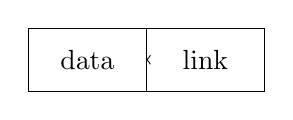
\begin{tikzpicture}
            \node[draw, rectangle, minimum width=1.5cm, minimum height=0.8cm] (data) {data};
            \node[draw, rectangle, minimum width=1.5cm, minimum height=0.8cm, right of=data, node distance=1.5cm] (link) {link};
            \draw[->] (data.east) -- (link.west);
        \end{tikzpicture}
        \end{center}
        假设该链表只给出了头指针 list。在不改变链表的前提下,请设计一个尽可能高效的算法,查找链表中倒数第 $k$ 个位置上的结点 ($k$ 为正整数)。若查找成功,算法输出该结点的 data 域的值,并返回 $1$;否则,只返回 $0$。要求:
        \begin{subqitems}
            \subqitem 描述算法的基本设计思想。
            \subqitem 描述算法的详细实现步骤。
            \subqitem 根据设计思想和实现步骤,采用程序设计语言描述算法 (使用 C、C++或 Java 语言实现),关键之处给出简要注释。
        \end{subqitems}
    \end{bbox}

    \begin{bbox}
        \qitem 【2012 统考真题】假设采用带头结点的单链表保存单词,当两个单词有相同的后缀时,可共享相同的后缀存储空间,例如,loading 和 being 的存储映像如下图所示。
        
        \imgin[1]{}{fig/fig2.3.18.png}

        设 str1 和 str2 分别指向两个单词所在单链表的头结点,链表结点结构为 [data] [link],请设计一个时间上尽可能高效的算法,找出由 str1 和 str2 所指向的两个链表共同后缀的起始位置 (如图中字符 i 所在结点的位置 p)。要求:
        \begin{subqitems}
            \subqitem 给出算法的基本设计思想。
            \subqitem 根据设计思想,采用 C 或 C++或 Java 语言描述算法,关键之处给出注释。
            \subqitem 说明你所设计算法的时间复杂度。
        \end{subqitems}
    \end{bbox}

    \begin{bbox}
        \qitem 【2015 统考真题】用单链表保存 $m$ 个整数,结点的结构为 [data] [link],且 |data| $\le n$ ($n$ 为正整数)。现要求设计一个时间复杂度尽可能高效的算法,对于链表中 data 的绝对值相等的结点,仅保留第一次出现的结点而删除其余绝对值相等的结点。例如,若给定的单链表 head 如下:
        
        \imgin[1]{}{fig/fig2.3.19.1.png}
        
        则删除结点后的 head 为
        
        \imgin[1]{}{fig/fig2.3.19.2.png}
        
        要求:
        \begin{subqitems}
            \subqitem 给出算法的基本设计思想。
            \subqitem 使用 C 或 C++语言,给出单链表结点的数据类型定义。
            \subqitem 根据设计思想,采用 C 或 C++语言描述算法,关键之处给出注释。
            \subqitem 说明你所设计算法的时间复杂度和空间复杂度。
        \end{subqitems}
    \end{bbox}

    \begin{bbox}
        \qitem 【2019 统考真题】设线性表 $L=(a_1,a_2,a_3,\dots,a_{n-2},a_{n-1},a_n)$ 采用带头结点的单链表保存,链表中的结点定义如下:
        \begin{lstlisting}[language=C, basicstyle=\ttfamily\small]
typedef struct node {
    int data;
    struct node*next;
}NODE;
        \end{lstlisting}
        请设计一个空间复杂度为 $O(1)$ 且时间上尽可能高效的算法,重新排列 $L$ 中的各结点,得到线性表 $L'=(a_1,a_n,a_2,a_{n-1},a_3,a_{n-2},\dots)$。要求:
        \begin{subqitems}
            \subqitem 给出算法的基本设计思想。
            \subqitem 根据设计思想,采用 C 或 C++语言描述算法,关键之处给出注释。
            \subqitem 说明你所设计算法的时间复杂度。
        \end{subqitems}
    \end{bbox}

\end{qitems} 

% \setcounter{section}{2} 
% \section{栈、队列和数组}
% \subsection{栈}\qanswerloc{73}

\begin{qitems}

    \begin{bbox}
        \qitem 有 5 个元素,其入栈次序为 A, B, C, D, E, 在各种可能的出栈次序中,第一个出栈元素为 C 且第二个出栈元素为 D 的出栈序列有哪几个?
    \end{bbox}

    \begin{bbox}
        \qitem 若元素的入栈序列为 A, B, C, D, E, 运用栈操作,能否得到出栈序列 B, C, A, E, D 和 D, B, A, C, E?为什么?
    \end{bbox}

    \begin{bbox}
        \qitem 栈的初态和终态均为空,以 I 和 O 分别表示入栈和出栈,则出入栈的操作序列可表示为由 I 和 O 组成的序列,可以操作的序列称为合法序列,否则称为非法序列。
        \begin{subqitems}
            \subqitem 下面所示的序列中哪些是合法的?
            
            A. IOIIOIOO \quad B. IOOIOIIO \quad C. IIIOIOIO \quad D. IIIOOIOO
            \subqitem 通过对 1) 的分析,写出一个算法,判定所给的操作序列是否合法。若合法,返回 \texttt{true}, 否则返回 \texttt{false} (假定被判定的操作序列已存入一维数组中)。
        \end{subqitems}
    \end{bbox}

    \begin{bbox}
        \qitem 设单链表的表头指针为 L, 结点结构由 data 和 next 两个域构成,其中 data 域为字符型。试设计算法判断该链表的全部 n 个字符是否中心对称。例如 xyx、xyyx 都是中心对称。
    \end{bbox}

    \begin{bbox}
        \qitem 设有两个栈 $S_1$、$S_2$ 都采用顺序栈方式,并共享一个存储区 $[0, \dots, \text{maxsize}-1]$,为了尽量利用空间,减少溢出的可能,可采用栈顶相向、迎面增长的存储方式。试设计 $S_1$、$S_2$ 有关入栈和出栈的操作算法。
    \end{bbox}

\end{qitems}

% \subsection{队列}\qanswerloc{87}

\begin{qitems}

    \begin{bbox}
        \qitem 若希望循环队列中的元素都能得到利用,则需设置一个标志域 \texttt{tag},并以 \texttt{tag} 的值为 0 或 1 来区分队首指针 \texttt{front} 和队尾指针 \texttt{rear} 相同时的队列状态是"空"还是"满"。试编写与此结构相应的入队和出队算法。
    \end{bbox}

    \begin{bbox}
        \qitem Q 是一个队列,S 是一个空栈,实现将队列中的元素逆置的算法。
    \end{bbox}

    \begin{bbox}
        \qitem 利用两个栈 S1 和 S2 来模拟一个队列,已知栈的 4 个运算定义如下:
        \begin{lstlisting}[language=C, basicstyle=\ttfamily\small]
Push(S,x);        // 元素 x 入栈 S
Pop(S,x);         // S 出栈并将出栈的值赋给 x
StackEmpty(S);    // 判断栈是否为空
StackOverflow(S); // 判断栈是否为满
        \end{lstlisting}
        如何利用栈的运算来实现该队列的 3 个运算 (形参由读者根据要求自己设计)?
        \begin{lstlisting}[language=C, basicstyle=\ttfamily\small]
Enqueue(x);       // 将元素 x 入队
Dequeue(x);       // 出队,并将出队元素存储在 x 中
QueueEmpty();     // 判断队列是否为空
        \end{lstlisting}
    \end{bbox}

    \begin{bbox}
        \qitem 【2019 统考真题】请设计一个队列,要求满足:1.初始时队列为空;2.入队时,允许增加队列占用空间;3.出队后,出队元素所占用的空间可重复使用,即整个队列所占用的空间只增不减;4.入队操作和出队操作的时间复杂度始终保持为 O(1)。请回答:
        \begin{subqitems}
            \subqitem 该队列是应选择链式存储结构,还是应选择顺序存储结构?
            \subqitem 画出队列的初始状态,并给出判断队空和队满的条件。
            \subqitem 画出第一个元素入队后的队列状态。
            \subqitem 给出入队操作和出队操作的基本过程。
        \end{subqitems}
    \end{bbox}

\end{qitems} 

% \setcounter{section}{4} 
% \section{树与二叉树}
% \subsection{树的基本概念}\qanswerloc{129}

\begin{qitems}

    \begin{bbox}
        \qitem 含有 $n$ 个结点的三叉树的最小高度是多少?
    \end{bbox}

    \begin{bbox}
        \qitem 已知一棵度为 4 的树中,度为 0, 1, 2, 3 的结点数分别为 14, 4, 3, 2,求该树的结点总数 $n$ 和度为 4 的结点个数,并给出推导过程。
    \end{bbox}

    \begin{bbox}
        \qitem 已知一棵度为 $m$ 的树中,有 $n_1$ 个度为 1 的结点,有 $n_2$ 个度为 2 的结点……有 $n_m$ 个度为 $m$ 的结点,问该树有多少个叶结点?
    \end{bbox}

\end{qitems} 
% \subsection{二叉树的概念}\qanswerloc{139}

\begin{qitems}

    \begin{bbox}
        \qitem 在一棵完全二叉树中,含有 $n_0$ 个叶结点,当度为 1 的结点数为 1 时,该树的高度是多少?当度为 1 的结点数为 0 时,该树的高度是多少?
    \end{bbox}

    \begin{bbox}
        \qitem 一棵有 $n$ 个结点的满二叉树有多少个分支结点和多少个叶结点?该满二叉树的高度是多少?
    \end{bbox}

    \begin{bbox}
        \qitem 已知完全二叉树的第 9 层有 240 个结点,则整个完全二叉树有多少个结点?有多少个叶结点?
    \end{bbox}

    \begin{bbox}
        \qitem 一棵高度为 $h$ 的满 $m$ 叉树有如下性质:根结点所在层次为第 1 层,第 $h$ 层上的结点都是叶结点,其余各层上每个结点都有 $m$ 棵非空子树,若按层次自顶向下,同一层自左向右,顺序从 1 开始对全部结点进行编号,试问:
        \begin{subqitems}
            \subqitem 各层的结点个数是多少?
            \subqitem 编号为 $i$ 的结点的双亲结点(若存在)的编号是多少?
            \subqitem 编号为 $i$ 的结点的第 $k$ 个孩子结点(若存在)的编号是多少?
            \subqitem 编号为 $i$ 的结点的有右兄弟的条件是什么?其右兄弟结点的编号是多少?
        \end{subqitems}
    \end{bbox}

    \begin{bbox}
        \qitem 已知一棵二叉树按顺序存储结构进行存储,设计一个算法,求编号分别为 $i$ 和 $j$ 的两个结点的最近的公共祖先结点的值。
    \end{bbox}
    
    \begin{bbox}
        \qitem 【2016 统考真题】若一棵非空 $k$($k \ge 2$)叉树 $T$ 中的每个非叶结点都有 $k$ 个孩子,则称 $T$ 为正则 $k$ 叉树。请回答下列问题并给出推导过程。
        \begin{subqitems}
            \subqitem 若 $T$ 有 $m$ 个非叶结点,则 $T$ 中的叶结点有多少个?
            \subqitem 若 $T$ 的高度为 $h$ (单结点的树 $h=1$),则 $T$ 的结点数最多为多少个?最少为多少个?
        \end{subqitems}
    \end{bbox}

\end{qitems} 
% \subsection{二叉树的遍历和线索二叉树}\qanswerloc{161}

\begin{qitems}

    \begin{bbox}
        \qitem 若某非空二叉树的先序序列和后序序列正好相反,则该二叉树的形态是什么?
    \end{bbox}
    
    \begin{bbox}
        \qitem 若某非空二叉树的先序序列和后序序列正好相同,则该二叉树的形态是什么?
    \end{bbox}

    \begin{bbox}
        \qitem 假设二叉树采用二叉链表存储结构,设计一个非递归算法求二叉树的高度。
    \end{bbox}

    \begin{bbox}
        \qitem 二叉树按二叉链表形式存储,试编写一个判别给定二叉树是否是完全二叉树的算法。
    \end{bbox}

    \begin{bbox}
        \qitem 假设二叉树采用二叉链表存储结构存储,试设计一个算法,计算一棵给定二叉树的所有双分支结点个数。
    \end{bbox}
    
    \begin{bbox}
        \qitem 设树 B 是一棵采用链式结构存储的二叉树,编写一个把树 B 中所有结点的左、右子树进行交换的函数。
    \end{bbox}

    \begin{bbox}
        \qitem 假设二叉树采用二叉链表存储结构存储,设计一个算法,求先序遍历序列中第 $k$ ($1 \le k \le$ 二叉树中结点个数) 个结点的值。
    \end{bbox}

    \begin{bbox}
        \qitem 已知二叉树以二叉链表存储,编写算法完成:对于树中每个元素值为 $x$ 的结点,删除以它为根的子树,并释放相应的空间。
    \end{bbox}

    \begin{bbox}
        \qitem 在二叉树中查找值为 $x$ 的结点,试编写算法(用 C 语言)打印值为 $x$ 的结点的所有祖先,假设值为 $x$ 的结点不多于一个。
    \end{bbox}

    \begin{bbox}
        \qitem 设一棵二叉树的结点结构为 (LLINK, INFO, RLINK),ROOT 为指向该二叉树根结点的指针,$p$ 和 $q$ 分别为指向该二叉树中任意两个结点的指针,试编写算法 ANCESTOR(ROOT, $p, q, r$),找到 $p$ 和 $q$ 的最近公共祖先结点 $r$。
    \end{bbox}

    \begin{bbox}
        \qitem 假设二叉树采用二叉链表存储结构,设计一个算法,求非空二叉树 $b$ 的宽度(具有结点数最多的那一层的结点个数)。
    \end{bbox}

    \begin{bbox}
        \qitem 设有一棵满二叉树(所有结点值均不同),已知其先序序列为 \textit{pre},设计一个算法求其后序序列 \textit{post}。
    \end{bbox}

    \begin{bbox}
        \qitem 设计一个算法将二叉树的叶结点按从左到右的顺序连成一个单链表,表头指针为 \texttt{head}。二叉树按二叉链表方式存储,链接时用叶结点的右指针域来存放单链表指针。
    \end{bbox}

    \begin{bbox}
        \qitem 试设计判断两棵二叉树是否相似的算法。所谓二叉树 $T_1$ 和 $T_2$ 相似,指的是 $T_1$ 和 $T_2$ 都是空的二叉树或都只有一个根结点;或者 $T_1$ 的左子树和 $T_2$ 的左子树是相似的,且 $T_1$ 的右子树和 $T_2$ 的右子树是相似的。
    \end{bbox}

    \begin{bbox}
        \qitem 【2014 统考真题】二叉树的带权路径长度 (WPL) 是二叉树中所有叶结点的带权路径长度之和。给定一棵二叉树 $T$,采用二叉链表存储,结点结构为
        \begin{center}
            \begin{tabular}{|c|c|c|}
            \hline
            \texttt{left} & \texttt{weight} & \texttt{right} \\
            \hline
            \end{tabular}
        \end{center}
        其中叶结点的 \texttt{weight} 域保存该结点的非负权值。设 \texttt{root} 为指向 $T$ 的根结点的指针,请设计求 $T$ 的 WPL 的算法,要求:
        \begin{subqitems}
            \subqitem 给出算法的基本设计思想。
            \subqitem 使用 C 或 C++语言,给出二叉树结点的数据类型定义。
            \subqitem 根据设计思想,采用 C 或 C++语言描述算法,关键之处给出注释。
        \end{subqitems}
    \end{bbox}

    \begin{bbox}
        \qitem 【2017 统考真题】请设计一个算法,将给定的表达式树 (二叉树) 转换为等价的中缀表达式 (通过括号反映操作符的计算次序) 并输出。例如,当下列两棵表达式树作为算法的输入时:
        
        \begin{center}
            \begin{forest}
              for tree={circle, draw, s sep=10mm, l sep=5mm,},
              [*,
                [+,
                  [a]
                  [b]
                ]
                [*,
                  [c]
                  [-,
                    [,phantom]
                    [d]
                  ]
                ]
              ]
            \end{forest}
            \hspace{2cm}
            \begin{forest}
              for tree={circle, draw, s sep=15mm, l sep=8mm,},
              [+,
                [*,
                  [a]
                  [b]
                ]
                [-,
                  [-,
                    [c]
                    [d]
                  ]
                ]
              ]
            \end{forest}
        \end{center}
        
        输出的等价中缀表达式分别为 \texttt{(a+b)*(c*(-d))} 和 \texttt{(a*b)+(-(c-d))}。
        
        二叉树结点定义如下:
        \begin{lstlisting}[language=C, basicstyle=\ttfamily\small]
typedef struct node{
    char data[10];      // 存储操作数或操作符
    struct node *left, *right;
}BTree;
        \end{lstlisting}
        要求:
        \begin{subqitems}
            \subqitem 给出算法的基本设计思想。
            \subqitem 根据设计思想,采用 C 或 C++语言描述算法,关键之处给出注释。
        \end{subqitems}
    \end{bbox}

    \begin{bbox}
        \qitem 【2022 统考真题】已知非空二叉树 $T$ 的结点值均为正整数,采用顺序存储方式保存,数据结构定义如下:
        \begin{lstlisting}[language=C, basicstyle=\ttfamily\small]
typedef struct {              //MAX_SIZE 为已定义常量
    int SqBiTNode[MAX_SIZE];  //保存二叉树结点值的数组
    int ElemNum;              //实际占用的数组元素个数
} SqBiTree;
        \end{lstlisting}
        $T$ 中不存在的结点在数组 \texttt{SqBiTNode} 中用 -1 表示。例如,对于下图所示的两棵非空二叉树 $T_1$ 和 $T_2$:
        
        \begin{center}
            \begin{minipage}{0.45\linewidth}
                \centering
                \begin{forest}
                  for tree={circle, draw, l sep=8mm},
                  [40,
                    [25,
                      [, phantom]
                      [30,
                        [27]
                        [, phantom]
                      ]
                    ]
                    [60,
                      [, phantom]
                      [80]
                    ]
                  ]
                \end{forest}
                \\ 二叉树 $T_1$
            \end{minipage}
            \begin{minipage}{0.45\linewidth}
                \centering
                \begin{forest}
                  for tree={circle, draw, l sep=10mm, s sep=5mm},
                  [40,
                    [50,
                      [, phantom]
                      [30,
                        [, phantom]
                        [35]
                      ]
                    ]
                    [60]
                  ]
                \end{forest}
                \\ 二叉树 $T_2$
            \end{minipage}
        \end{center}
        
        \noindent $T_1$ 的存储结果如下: \\
        \texttt{T1.SqBiTNode} \hspace{1cm}
        \begin{tabular}{|c|c|c|c|c|c|c|c|c|c|}
        \hline
        40 & 25 & 60 & -1 & 30 & -1 & 80 & -1 & -1 & 27 \\
        \hline
        \end{tabular} \\
        \texttt{T1.ElemNum=10}
    
        \vspace{5mm}
    
        \noindent $T_2$ 的存储结果如下: \\
        \texttt{T2.SqBiTNode} \hspace{1cm}
        \begin{tabular}{|c|c|c|c|c|c|c|c|c|c|c|}
        \hline
        40 & 50 & 60 & -1 & 30 & -1 & -1 & -1 & -1 & -1 & 35 \\
        \hline
        \end{tabular} \\
        \texttt{T2.ElemNum=11}
    
        \vspace{5mm}
    
        \noindent 请设计一个尽可能高效的算法,判定一棵采用这种方式存储的二叉树是否为二叉搜索树,若是,则返回 \texttt{true},否则,返回 \texttt{false}。要求:
        \begin{subqitems}
            \subqitem 给出算法的基本设计思想。
            \subqitem 根据设计思想,采用 C 或 C++语言描述算法,关键之处给出注释。
        \end{subqitems}
    \end{bbox}

\end{qitems} 
% \subsection{树、森林}\qanswerloc{181}

\begin{qitems}
    \begin{bbox}
        \qitem 给定一棵树的先根遍历序列和后根遍历序列,能否唯一确定一棵树?若能,请举例说明;若不能,请给出反例。
    \end{bbox}

    \begin{bbox}
        \qitem 将下面一个由 3 棵树组成的森林转换为二叉树。
        \begin{center}
            \begin{forest}
                for tree={circle, draw, l=1.5cm},
                [A,
                    [B]
                    [C]
                ]
            \end{forest}
            \hspace{1cm}
            \begin{forest}
                for tree={circle, draw},
                [D,
                    [E,
                        [F]
                    ]
                ]
            \end{forest}
            \hspace{1cm}
            \begin{forest}
                for tree={circle, draw, l=1.5cm},
                [G,
                    [H,
                        [K]
                        [L]
                    ]
                    [I]
                    [J,
                        [M,
                            [P]
                        ]
                        [N]
                        [O]
                    ]
                ]
            \end{forest}
        \end{center}
    \end{bbox}

    \begin{bbox}
        \qitem 已知某二叉树的先序序列和中序序列分别为 \texttt{ABDEHCFIMGJKL} 和 \texttt{DBHEAIMFGCKLJ},请画出这棵二叉树,并画出二叉树对应的森林。
    \end{bbox}

    \begin{bbox}
        \qitem 编程求以孩子兄弟表示法存储的森林的叶结点数。
    \end{bbox}

    \begin{bbox}
        \qitem 以孩子兄弟链表为存储结构,请设计递归算法求树的深度。
    \end{bbox}

\end{qitems} 
% \subsection{树与二叉树的应用}\qanswerloc{194}

\begin{qitems}
    \begin{bbox}
        \qitem 设给定权集 $w = \{5, 7, 2, 3, 6, 8, 9\}$,试构造关于 $w$ 的一棵哈夫曼树,并求其加权路径长度 WPL。
    \end{bbox}

    \begin{bbox}
        \qitem 【2012 统考真题】设有 6 个有序表 A, B, C, D, E, F,分别含有 10, 35, 40, 50, 60 和 200 个数据元素,各表中的元素按升序排列。要求通过 5 次两两合并,将 6 个表最终合并为 1 个升序表,并使最坏情况下比较的总次数达到最小。请回答下列问题:
        \begin{subqitems}
            \subqitem 给出完整的合并过程,并求出最坏情况下比较的总次数。
            \subqitem 根据你的合并过程,描述 $n(n \ge 2)$ 个不等长升序表的合并策略,并说明理由。
        \end{subqitems}
    \end{bbox}

    \begin{bbox}
        \qitem 【2020 统考真题】若任意一个字符的编码都不是其他字符编码的前缀,则称这种编码具有前缀特性。现有某字符集(字符个数 $\ge 2$)的不等长编码,每个字符的编码均为二进制的 0、1 序列,最长为 $L$ 位,且具有前缀特性。请回答下列问题:
        \begin{subqitems}
            \subqitem 哪种数据结构适宜保存上述具有前缀特性的不等长编码?
            \subqitem 基于你所设计的数据结构,简述从 0/1 串到字符串的译码过程。
            \subqitem 简述判定某字符集的不等长编码是否具有前缀特性的过程。
        \end{subqitems}
    \end{bbox}

\end{qitems} 

\setcounter{section}{5} 
\section{图}
\subsection{图的基本概念}\qanswerloc{205}

\begin{qitems}
    \begin{bbox}
        \qitem 图 $G$ 是一个非连通无向图,共有 28 条边,该图至少有多少个顶点?
    \end{bbox}
\end{qitems} 
\subsection{图的存储及基本操作}\qanswerloc{216}

\begin{qitems}
    \begin{bbox}
        \qitem 已知带权有向图 $G$ 的邻接矩阵如下图所示,请画出该带权有向图 $G$。
        \[
            \begin{pmatrix}
                0 & 15 & 2 & 12 & \infty & \infty & \infty \\
                \infty & 0 & \infty & \infty & 6 & \infty & \infty \\
                \infty & \infty & 0 & \infty & 8 & 4 & \infty \\
                \infty & \infty & \infty & 0 & \infty & \infty & 3 \\
                \infty & \infty & \infty & \infty & 0 & \infty & 9 \\
                \infty & \infty & 5 & \infty & \infty & 0 & 10 \\
                \infty & 4 & \infty & \infty & \infty & \infty & 0
            \end{pmatrix}
        \]
    \end{bbox}

    \begin{solution}
        该带权有向图如下图所示:
        \begin{center}
            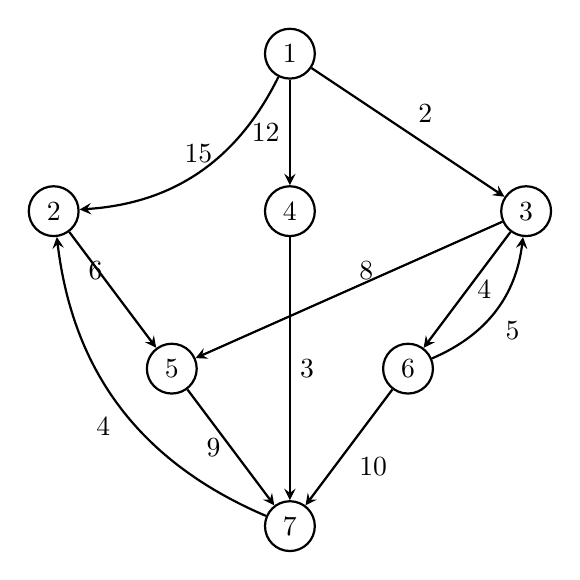
\begin{tikzpicture}[->, >=stealth, auto, node distance=2.5cm, thick]
                \tikzstyle{vertex}=[circle, draw, minimum size=18pt, inner sep=2pt]
                
                \node[vertex] (v1) at (0, 4) {1};
                \node[vertex] (v2) at (-3, 2) {2};
                \node[vertex] (v3) at (3, 2) {3};
                \node[vertex] (v4) at (0, 2) {4};
                \node[vertex] (v5) at (-1.5, 0) {5};
                \node[vertex] (v6) at (1.5, 0) {6};
                \node[vertex] (v7) at (0, -2) {7};
                
                \path (v1) edge[bend left] node[pos=0.5, above] {15} (v2);
                \path (v1) edge node[pos=0.5, above right] {2} (v3);
                \path (v1) edge node[pos=0.5, left] {12} (v4);
                \path (v2) edge node[pos=0.5, above left] {6} (v5);
                \path (v3) edge node[pos=0.5, above right] {8} (v5);
                \path (v3) edge node[pos=0.5, right] {4} (v6);
                \path (v4) edge node[pos=0.5, right] {3} (v7);
                \path (v5) edge node[pos=0.5, left] {9} (v7);
                \path (v6) edge[bend right] node[pos=0.5, below right] {5} (v3);
                \path (v6) edge node[pos=0.5, below right] {10} (v7);
                \path (v7) edge[bend left] node[pos=0.5, below left] {4} (v2);
            \end{tikzpicture}
        \end{center}
    \end{solution}

    \begin{bbox}
        \qitem 设图 $G = (V, E)$ 以邻接表存储,如下图所示。画出其邻接矩阵存储及图 $G$。
        \imgin[0.7]{}{fig/fig6.2.2.png}
    \end{bbox}

    \begin{solution}
        根据邻接表,该图是无向图,其邻接矩阵为:
        \[
            \begin{pmatrix}
                0 & 1 & 1 & 1 & 0 \\
                1 & 0 & 1 & 1 & 1 \\
                1 & 1 & 0 & 1 & 0 \\
                1 & 1 & 1 & 0 & 1 \\
                0 & 1 & 0 & 1 & 0
            \end{pmatrix}
        \]
        图 $G$ 如下图所示:
        \begin{center}
            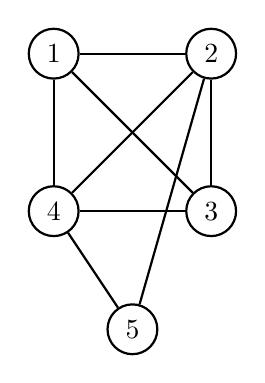
\begin{tikzpicture}[-, auto, node distance=2cm, thick]
                \tikzstyle{vertex}=[circle, draw, minimum size=18pt, inner sep=2pt]
                
                \node[vertex] (v1) at (0, 2) {1};
                \node[vertex] (v2) at (2, 2) {2};
                \node[vertex] (v3) at (2, 0) {3};
                \node[vertex] (v4) at (0, 0) {4};
                \node[vertex] (v5) at (1, -1.5) {5};
                
                \path (v1) edge (v2);
                \path (v1) edge (v3);
                \path (v1) edge (v4);
                \path (v2) edge (v3);
                \path (v2) edge (v4);
                \path (v2) edge (v5);
                \path (v3) edge (v4);
                \path (v4) edge (v5);
            \end{tikzpicture}
        \end{center}
    \end{solution}

    \begin{bbox}
        \qitem 对 $n$ 个顶点的无向图和有向图,分别采用邻接矩阵和邻接表表示时,试问:
        \begin{subqitems}
            \subqitem 如何判别图中有多少条边?
            \subqitem 如何判别任意两个顶点 $i$ 和 $j$ 是否有边相连?
            \subqitem 任意一个顶点的度是多少?
        \end{subqitems}
    \end{bbox}

    \begin{bbox}
        \qitem 如何对无环有向图中的顶点重新编号,使得该图的邻接矩阵中所有的 1 都集中到对角线以上?
    \end{bbox}

    \begin{bbox}
        \qitem 写出从图的邻接表表示转换成邻接矩阵表示的算法。
    \end{bbox}

    \begin{bbox}
        \qitem 【2015统考真题】已知有5个顶点的图G如下图所示。
        \imgin[0.6]{}{fig/fig6.2.6.png}
        \begin{subqitems}
            \subqitem 写出图G的邻接矩阵A(行、列下标从0开始)。
            \subqitem 求$A^2$,矩阵$A^2$中位于0行3列元素值的含义是什么?
            \subqitem 若已知具有n($n \ge 2$)个顶点的图的邻接矩阵为B,则$B^m$($2 \le m \le n$)中非零元素的含义是什么?
        \end{subqitems}
    \end{bbox}

    \begin{bbox}
        \qitem 【2021统考真题】已知无向连通图 $G$ 顶点集为 $V$ 和边集 $E$ 组成,$|E|>0$。当 $G$ 中度为奇数的顶点个数为不大于2的偶数时,G 存在包含所有边且长度为 $|E|$ 的路径(称为 EL 路径)。设图 $G$ 采用邻接矩阵存储,类型定义如下:
        \begin{lstlisting}[language=C, basicstyle=\ttfamily\small]
typedef struct {
    int numVertices, numEdges;  //图中实际的顶点数和边数
    char VerticesList[MAXV];    //顶点表, MAXV为已定义常量
    int Edge[MAXV][MAXV];       //邻接矩阵
} MGraph;
        \end{lstlisting}
        请设计算法 \lstinline{int IsExistEL(MGraph G)},判断 G 是否存在 EL 路径,若存在,则返回1,否则返回0。要求:
        \begin{subqitems}
            \subqitem 给出算法的基本设计思想。
            \subqitem 根据设计思想,采用C或C++语言描述算法,关键之处给出注释。
            \subqitem 说明你所设计算法的时间和空间复杂度。
        \end{subqitems}
    \end{bbox}
 
    \begin{bbox}
            \qitem 【2023统考真题】已知有向图G采用邻接矩阵存储,类型定义如下:
            \begin{lstlisting}[language=C, basicstyle=\ttfamily\small]
typedef struct {
    int numVertices, numEdges;  //图的顶点数和有向边数
    char VerticesList[MAXV];    //顶点表, MAXV为已定义常量
    int Edge[MAXV][MAXV];       //邻接矩阵
} MGraph;
            \end{lstlisting}
            将图中出度大于入度的顶点称为K顶点。例如,在下图中,顶点a和b为K顶点。
            \imgin[0.6]{}{fig/fig6.2.8.png}

            请设计算法 \lstinline{int printVertices(MGraph G)},对给定的任意非空有向图G,输出G中所有的K顶点,并返回K顶点的个数。要求:
            \begin{subqitems}
                \subqitem 给出算法的基本设计思想。
                \subqitem 根据设计思想,采用C或C++语言描述算法,关键之处给出注释。
            \end{subqitems}
    \end{bbox}
    
\end{qitems} 
\subsection{图的遍历}\qanswerloc{228}
\begin{qitems}
    \begin{bbox}
        \qitem 图 $G=(V,E)$ 以邻接表存储,如下图所示,试画出图 G 的深度优先生成树和广度优先生成树(假设从结点 1 开始遍历)。
        \imgin[0.8]{}{fig/fig6.3.1.png}
    \end{bbox}

    \begin{bbox}
        \qitem 给定一个连通无向图,将图的所有顶点分别染成红色或蓝色,若存在一种染色方法使图中每条边的两个顶点的颜色都不同,则称这个图能被二分。对于下图所示的两个无向图:
        \imgin[0.6]{}{fig/fig6.3.2.png}
        \begin{subqitems}
            \subqitem 判断上面两个无向图是否能被二分,若能二分,则请标出每个顶点的颜色。
            \subqitem 请设计一种算法来判断是否能被二分,仅用语言描述算法的思想即可。
            \subqitem 给出你设计的算法的时间复杂度和空间复杂度。
        \end{subqitems}
    \end{bbox}
    \begin{bbox}
        \qitem 试设计一个算法,判断一个无向图 G 是否为一棵树。若是,则算法返回 true,否则返回 false。
    \end{bbox}

    \begin{bbox}
        \qitem 分别采用基于深度优先遍历和广度优先遍历算法判别以邻接表方式存储的有向图中是否存在由顶点 $v_i$ 到顶点 $v_j$ 的路径($i \neq j$)。注意,算法中涉及的图的基本操作必须在此存储结构上实现。
    \end{bbox}

    \begin{bbox}
        \qitem 假设图用邻接表表示,设计一个算法,输出从顶点 $V_i$ 到顶点 $V_j$ 的所有简单路径。
    \end{bbox}
\end{qitems}
\subsection{图的应用}\qanswerloc{259}
\begin{qitems}
    \begin{bbox}
        \qitem 下面是一种称为"破圈法"的求解最小生成树的方法:所谓"破圈法",是指"任取一圈,去掉圈上权最大的边",反复执行这一步骤,直到没有圈为止。试判断这种方法是否正确。若正确,说明理由;若不正确,举出反例(注:圈就是回路)。
    \end{bbox}
    \begin{bbox}
        \qitem 已知有向图如下图所示。
        \imgin[0.7]{}{fig/fig6.4.2.png}
        \begin{subqitems}
            \subqitem 写出该图的邻接矩阵表示并据此给出从顶点 1 出发的深度优先遍历序列。
            \subqitem 求该有向图的强连通分量的数目。
            \subqitem 给出该图的任意两个拓扑序列。
            \subqitem 若将该图视为无向图,分别用 Prim 算法和 Kruskal 算法求最小生成树。
        \end{subqitems}
    \end{bbox}
    \begin{bbox}
        \qitem 对下图所示的无向图,按照 Dijkstra 算法,写出从顶点 1 到其他各个顶点的最短路径和最短路径长度(顺序不能颠倒)。
        \imgin[0.8]{}{fig/fig6.4.3.png}
    \end{bbox}
    \begin{bbox}
        \qitem 下图所示为一个用 AOE 网表示的工程。
        \imgin[0.6]{}{fig/fig6.4.4.png}
        \begin{subqitems}
            \subqitem 画出此图的邻接表表示。
            \subqitem 完成此工程至少需要多少时间?
            \subqitem 指出关键路径。
            \subqitem 哪些活动加速可以缩短完成工程所需的时间?
        \end{subqitems}
    \end{bbox}
    \begin{bbox}
        \qitem 下表给出了某工程各工序之间的优先关系和各工序所需的时间(其中"—"表示无先驱工序),请完成以下各题:
        \begin{center}
        \begin{tabular}{|l|c|c|c|c|c|c|c|c|}
        \hline
        工序代号 & A & B & C & D & E & F & G & H \\
        \hline
        所需时间 & 3 & 2 & 2 & 3 & 4 & 3 & 2 & 1 \\
        \hline
        先驱工序 & --- & --- & A & A & B & A & C, E & D \\
        \hline
        \end{tabular}
        \end{center}
        \begin{subqitems}
            \subqitem 画出相应的 AOE 网。
            \subqitem 列出各事件的最早发生时间和最迟发生时间。
            \subqitem 求出关键路径并指明完成该工程所需的最短时间。
        \end{subqitems}
    \end{bbox}
    \begin{bbox}
        \qitem 试编写利用 DFS 实现有向无环图拓扑排序的算法。
    \end{bbox}
    \begin{bbox}
        \qitem 【2009 统考真题】带权图(权值非负,表示边连接的两顶点间的距离)的最短路径问题是找出从初始顶点到目标顶点之间的一条最短路径。假设从初始顶点到目标顶点之间存在路径,现有一种解决该问题的方法:\\
        \ding{172} 设最短路径初始时仅包含初始顶点,令当前顶点 $u$ 为初始顶点。\\
        \ding{173} 选择离 $u$ 最近且尚未在最短路径中的一个顶点 $v$,加入最短路径,修改当前顶点 $u=v$。\\
        \ding{174} 重复步骤\ding{173},直到 $u$ 是目标顶点时为止。\\
        请问上述方法能否求得最短路径?若该方法可行,请证明;否则,请举例说明。
    \end{bbox}
    \begin{bbox}
        \qitem 【2011 统考真题】已知有 6 个顶点(顶点编号为 0$\sim$5)的有向带权图 G,其邻接矩阵 A 为上三角矩阵,按行为主序(行优先)保存在如下的一维数组中。
        \begin{center}
        \begin{tabular}{|c|c|c|c|c|c|c|c|c|c|c|c|c|c|c|}
        \hline
        4 & 6 & $\infty$ & $\infty$ & $\infty$ & 5 & $\infty$ & $\infty$ & $\infty$ & 4 & 3 & $\infty$ & $\infty$ & 3 & 3 \\
        \hline
        \end{tabular}
        \end{center}
        要求:
        \begin{subqitems}
            \subqitem 写出图 G 的邻接矩阵 A。
            \subqitem 画出有向带权图 G。
            \subqitem 求图 G 的关键路径,并计算该关键路径的长度。
        \end{subqitems}
    \end{bbox}
    \begin{bbox}
        \qitem 【2014 统考真题】某网络中的路由器运行 OSPF 路由协议,下表是由路由器 R1 维护的主要链路状态信息(LSI),R1 构造的网络拓扑图(见下图)是根据题下表及 R1 的接口名构造出来的网络拓扑。
        \imgin[0.6]{}{fig/fig6.4.10.png}
        请回答下列问题。
        \begin{subqitems}
            \subqitem 本题中的网络可抽象为数据结构中的哪种逻辑结构?
            \subqitem 针对表中的内容,设计合理的链式存储结构,以保存表中的链路状态信息(LSI)。要求给出链式存储结构的数据类型定义,并画出对应表的链式存储结构示意图(示意图中可以仅以 ID 标识结点)。
            \subqitem 按照 Dijkstra 算法的策略,依次给出 R1 到达子网 192.1.x.x 的最短路径及费用。
        \end{subqitems}
    \end{bbox}
    \begin{bbox}
        \qitem 【2017 统考真题】使用 Prim 算法求带权连通图的最小(代价)生成树(MST)。请回答下列问题:
        \imgin[0.7]{}{fig/fig6.4.11.png}
        \begin{subqitems}
            \subqitem 对下列图 G,从顶点 A 开始求 G 的 MST,依次给出按算法选出的边。
            \subqitem 图 G 的 MST 是唯一的吗?
            \subqitem 对任意的带权连通图,满足什么条件时,其 MST 是唯一的?
        \end{subqitems}
    \end{bbox}
    \begin{bbox}
        \qitem 【2018 统考真题】拟建设一个光通信骨干网络连通 BJ、CS、XA、QD、JN、NJ、TL 和 WH 等 8 个城市,下图中无向边上的权值表示两个城市之间备选光缆的铺设费用。
        \imgin[0.7]{}{fig/fig6.4.12.png}
        请回答下列问题:
        \begin{subqitems}
            \subqitem 仅从铺设费用角度出发,给出所有可能的最经济的光缆铺设方案(用带权图表示),并计算相应方案的总费用。
            \subqitem 该图可采用图的哪种存储结构?给出求解问题 1)所用的算法名称。
            \subqitem 假设每个城市采用一个路由器按 1)中得到的最经济方案组网,主机 H1 直接连接 TL 的路由器,主机 H2 直接连接 BJ 的路由器。若 H1 向 H2 发送一个 TTL = 5 的 IP 分组,则 H2 是否可以收到该 IP 分组?
        \end{subqitems}
    \end{bbox}
    \begin{bbox}
        \qitem 【2024 统考真题】2023 年 10 月 26 日,神舟十七号载人飞船发射取得圆满成功,再次彰显了中国航天事业的辉煌成就。载人航天工程是包含众多子工程的复杂系统工程,为了保证工程的有序开展,需要明确各子工程的前导子工程,以协调各子工程的实施。该问题可以简化、抽象为有向图的拓扑序列问题。已知有向图 G 采用邻接矩阵存储,类型定义如下。
        \begin{lstlisting}[language=C, basicstyle=\ttfamily\small]
typedef struct {                //图的类型定义
    int numVertices, numEdges;  //图的顶点数和有向边数
    char VerticesList[MAXV];    //顶点表, MAXV为已定义常量
    int Edge[MAXV][MAXV];       //邻接矩阵
} MGraph;
        \end{lstlisting}
        请设计算法:\lstinline{int uniquely(MGraph G)},判定 G 是否存在唯一的拓扑序列,若是,则返回 1,否则返回 0。要求如下。
        \begin{subqitems}
            \subqitem 给出算法的基本设计思想。
            \subqitem 根据设计思想,采用 C 或 C++语言描述算法,关键之处给出注释。
        \end{subqitems}
    \end{bbox}
\end{qitems} 



% 确保最终为偶数页
\AtEndDocument{%
  \clearpage
  \edef\lastpage{\getpagerefnumber{LastPage}}
  \ifodd\lastpage
    \null\thispagestyle{empty}\newpage
  \fi
}

\end{document}